\documentclass[11pt, spanish]{article}
\usepackage[T1]{fontenc}
\usepackage[utf8]{inputenc}
\usepackage{amsmath}
\usepackage{amssymb}
% \usepackage{hyperref}
\usepackage{graphicx}
\usepackage{tikz}
\usetikzlibrary{shapes,arrows,positioning,calc}
\usepackage{geometry}
\geometry{
	left=15mm,
	right=15mm,
	top=5mm,
	bottom=20mm,
}

\tikzset{
block/.style = {draw, fill=white, rectangle, minimum height=3em, minimum width=3em},
tmp/.style  = {coordinate}, 
sum/.style= {draw, fill=white, circle, node distance=1cm},
input/.style = {coordinate},
output/.style= {coordinate},
pinstyle/.style = {pin edge={to-,thin,black}
}
}
\title{Control de Sistemas - Examen Parcial - Solución}
\author{Pontificia Universidad Javeriana, Bogotá\\Profesor: Ing. Gerardo Becerra, Ph.D.}
\date{Marzo 10 de 2020}

\begin{document}
	\maketitle
		\begin{description}
			\item 1. El sistema de control de posición de la plataforma de una aeronave está governada por las siguientes ecuaciones:
			\begin{align}
				\frac{d^2p(t)}{dt^2} + 2 \frac{dp(t)}{dt} + 4p(t) = \theta(t)\\
				\frac{d\theta(t)}{dt} = 0.5v_2(t)\\
				v_1(t) = r(t) - p(t)\\
				v_2(t) = 8v_1(t)
			\end{align}
			Las variables involucradas son las siguientes:
			\begin{itemize}
				\item $r(t)$: posición deseada de la plataforma.
				\item $p(t)$: posición real de la plataforma.
				\item $v_1(t)$: señal de error.
				\item $v_2(t)$: señal de error amplificada.
				\item $\theta(t)$: posición del eje del motor.
			\end{itemize}
			\begin{description}
				\item a. Obtenga el diagrama de bloques del sistema, identificando claramente todos los elementos (subsistemas, señales, etc).\\
				% \vspace*{3mm}
				Usando la notación de punto para representar las derivadas respecto al tiempo, se reescriben las ecuaciones de la siguiente forma:
				\begin{subequations}
					\begin{align}
						\ddot{p}(t) &= -2 \dot{p}(t) - 4p(t) + \theta(t)\\
						\dot{\theta}(t) &= 0.5 v_2(t)\\
						v_1(t) &= r(t) - p(t)\\
						v_2(t) &= 8v_1(t)
					\end{align}
					\label{eq:prob1_sistequ}
				\end{subequations}
				En la Fig. \ref{fig:prob1_diagbloques} se muestra el diagrama en bloques que representa el sistema de Ecs. \ref{eq:prob1_sistequ}.
				\begin{figure}
					\centering
					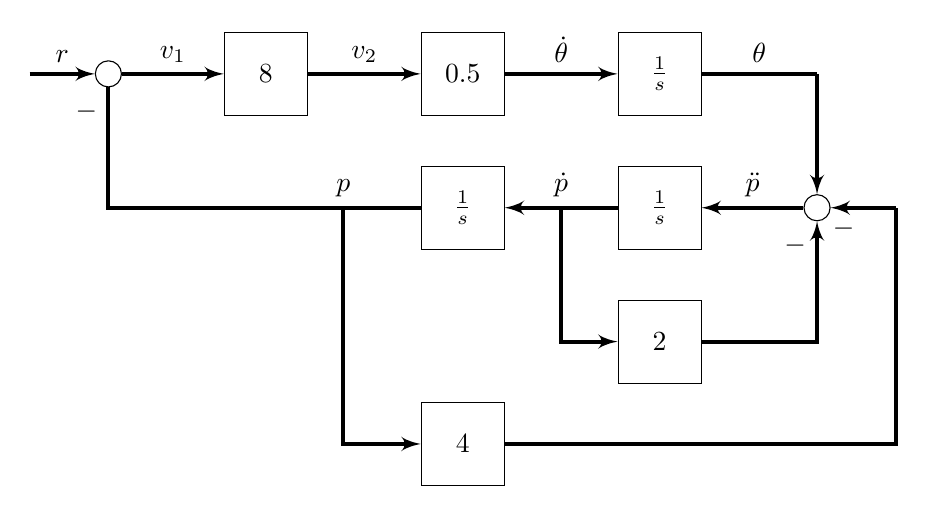
\begin{tikzpicture}[auto, node distance=2.5cm,>=latex']
						\node[input, name=rinput] (rinput) {};
						\node[sum, right of=rinput] (sum1) {};
						\node[block, right of=sum1,node distance=2cm] (amplifier) {8};
						\node[block, right of=amplifier] (motorgain) {0.5};
						\node[block, right of=motorgain] (thetadotint) {$\frac{1}{s}$};
						\node[block, below of=thetadotint,node distance=1.7cm] (pddotint) {$\frac{1}{s}$};
						\node[block, below of=motorgain,node distance=1.7cm] (pdotint) {$\frac{1}{s}$};
						\node[block, below of=pddotint,node distance=1.7cm] (gain1) {2};
						\node[block, below of=pdotint,node distance=3cm] (gain2) {4};
						\node[output, right of=thetadotint, node distance=2cm] (output) {};
						\node[sum, right of=pddotint, node distance=2cm] (sum2) {};
					  \node[tmp, below of=amplifier, node distance=1.7cm] (tmp1){};
					  \node[tmp, right of=sum2, node distance=1cm] (tmp2){};
						\draw[->,line width = 0.5mm] (rinput) -- node{$r$} (sum1);
						\draw[->,line width = 0.5mm] (sum1) -- node[name=v1,anchor=south]{$v_1$} (amplifier);
						\draw[->,line width = 0.5mm] (amplifier) -- node[name=v2,anchor=south]{$v_2$} (motorgain);
						\draw[->,line width = 0.5mm] (motorgain) -- node[name=thetadot,anchor=south]{$\dot{\theta}$} (thetadotint);
						\draw[line width=0.5mm] (thetadotint) -- node[name=theta,anchor=south] {$\theta$} (output);
						\draw[->,line width=0.5mm] (sum2) -- node[name=pddot,anchor=south] {$\ddot{p}$} (pddotint);
						\draw[->,line width=0.5mm] (pddotint) -- node[name=pdot,anchor=south] {$\dot{p}$} (pdotint);
						\draw[line width=0.5mm] (pdotint) -- node[name=p,anchor=south] {$p$} (tmp1);
						\draw[line width=0.5mm] (tmp1) -| node[pos=0.9] {$-$} (sum1);
						\draw[->,line width=0.5mm] (output) -- (sum2);
						\draw[->,line width=0.5mm] (pdot) |- (gain1);
						\draw[->,line width=0.5mm] (gain1) -| node[pos=0.9] {$-$} (sum2);
						\draw[->,line width=0.5mm] (p) |- (gain2);
						\draw[line width=0.5mm] (gain2) -| (tmp2);
						\draw[->,line width=0.5mm] (tmp2) -- node[pos=0.8] {$-$} (sum2);
					\end{tikzpicture}
					\caption{Diagrama en bloques para el problema 1.}
					\label{fig:prob1_diagbloques}
				\end{figure}

				\item b. Obtenga la representación en variables de estado del sistema.\\
				Para encontrar la representación en variables de estado, se realiza un cambio de variable:
				\begin{align*}
					x_1(t) &= p(t) \Rightarrow \dot{x}_1(t) = \dot{p}(t)\\
					x_2(t) &= \dot{x}_1(t) = \dot{p}(t)\\
					x_3(t) &= \theta(t)
				\end{align*}
				Reemplazando en las Ecs. \ref{eq:prob1_sistequ} se obtiene:
				\begin{align*}
					\dot{x}_1(t) &= x_2(t)\\
					\dot{x}_2(t) &= -4x_1(t) -2x_2(t) + x_3(t)\\
					\dot{x}_3(t) &= -4x_1(t) + 4r(t)
				\end{align*}
				Reescribiendo éstas ecuaciones en forma matricial se obtiene la ecuación de estado:
				\begin{equation*}
					\begin{bmatrix}
						\dot{x}_1(t)\\ \dot{x}_2(t)\\ \dot{x}_3(t) 
					\end{bmatrix} = 
					\begin{bmatrix}
						 0 &  1 & 0\\
						-4 & -2 & 1\\
						-4 &  0 & 0
					\end{bmatrix}
					\begin{bmatrix}
						x_1(t)\\ x_2(t)\\ x_3(t) 
					\end{bmatrix} +
					\begin{bmatrix}
						0 \\ 0 \\ 4
					\end{bmatrix} r(t)
				\end{equation*}
			\end{description}
			
			\item 2. Un sistema de control con retroalimentación negativa unitaria posee la siguiente función de lazo abierto:
			\begin{equation*}
				G_c(s)G(s) = \frac{K}{s(s+\sqrt{2K})}
			\end{equation*}
			\begin{description}
				\item a. Determine el porcentaje de sobrepico y tiempo de establecimiento (criterio de 2\%) de la respuesta debida a una entrada paso unitaria.\\
				La función de transferencia de lazo cerrado es:
				\begin{equation*}
					G_{cl}(s) = \frac{\frac{K}{s^2+\sqrt{2K}s}}{1+\frac{K}{s^2+\sqrt{2K}s}} = \frac{K}{s^2+\sqrt{2K}+K}
				\end{equation*}
				Note que la función de lazo abierto tiene la forma ideal de un sistema de segundo orden:
				\begin{equation*}
					G_{cl}(s) = \frac{\omega_n^2}{s^2 + 2\zeta \omega_n s + \omega_n^2}
				\end{equation*}
				Entonces, los valores de $\zeta$ y $\omega_n$ se obtienen:
				\begin{align*}
					\omega_n^2 &= K \Rightarrow \omega_n = \sqrt{K}\\
					2\zeta \omega_n &= \sqrt{2K} \Rightarrow \zeta = \frac{\sqrt{2K}}{2\omega_n} = \frac{\sqrt{2K}}{2\sqrt{K}} = \frac{\sqrt{2}}{2}
				\end{align*}
				El porcentaje de sobrepico es:
				\begin{equation*}
					PO = 100e^{-\pi \zeta/\sqrt{1-\zeta^2}} = 100e^{-\pi (\sqrt{2}/2) / \sqrt{1-(\sqrt{2}/2})^2} = 100e^{-\pi (\sqrt{2}/2) / (1/\sqrt{2})} = 100e^{-\pi}
				\end{equation*}
				El tiempo de establecimiento es:
				\begin{equation*}
					T_s = \frac{4}{\zeta \omega_n} = \frac{4}{\frac{\sqrt{2}}{2}\sqrt{K}} = \frac{4\sqrt{2}}{\sqrt{K}}
				\end{equation*}

				\item b. Para qué rango de $K$ se tiene $T_s \leq 1$ s?\\
				\begin{equation*}
					T_s \leq 1 \Rightarrow \frac{4\sqrt{2}}{\sqrt{K}} \leq 1 \Rightarrow 4\sqrt{2} \leq \sqrt{K} \Rightarrow K \geq 32
				\end{equation*}
			\end{description}
			
			\item 3. Considere el sistema mostrado en la Fig. \ref{fig:blockDiagram}(a).
			\begin{description}
				\item a. Determine $G(s)$ y $H(s)$ del diagrama de bloques mostrado en la Fig. \ref{fig:blockDiagram}(b) que son equivalentes a los del diagrama de la Fig. \ref{fig:blockDiagram}(a).\\
				Para simplificar el diagrama de bloques la señal que se realimenta unitariamente en la primera suma se puede mover a $Y(s)$. En ese caso el diagrama queda como el mostrado en la Fig. \ref{fig:blockDiagramSimplification}(a). Luego, utilizando operaciones fundamentales se simplifica la realimentación en \ref{fig:blockDiagramSimplification}(b) y se obtiene la cascada en \ref{fig:blockDiagramSimplification}(c). Por lo tanto, se tiene que
				\begin{equation*}
					G(s) = \frac{1}{(s+5)(s+11)}, \hspace*{3mm} H(s) = s+10
				\end{equation*}

				\item b. Determine $Y(s)/R(s)$ para la Fig. \ref{fig:blockDiagram}(b).\\
				La función de transferencia total se obtiene como:
				\begin{align*}
					\frac{Y(s)}{R(s)} &= \frac{G(s)}{1+G(s)H(s)} = \frac{\frac{1}{(s+5)(s+11)}}{1+\frac{(s+10)}{(s+5)(s+11)}} = \frac{1}{(s+5)(s+11)+(s+10)}\\
					&= \frac{1}{s^2+17s+65}
				\end{align*}

			\end{description}
			\begin{figure}
				\centering
				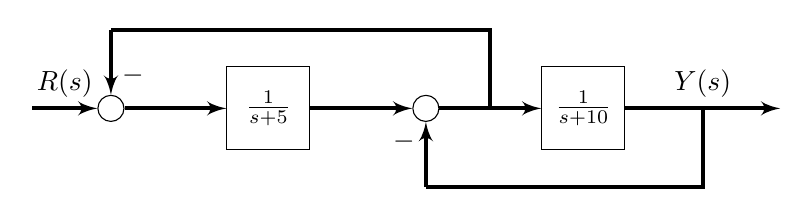
\begin{tikzpicture}[auto, node distance=2.5cm,>=latex']
					\node[input, name=rinput] (rinput) {};
					\node[sum, right of=rinput] (sum1) {};
					\node[block, right of=sum1,node distance=2cm] (sys1) {$\frac{1}{s+5}$};
					\node[sum, right of=sys1,node distance=2cm] (sum2) {};
					\node[block, right of=sum2,node distance=2cm] (sys2) {$\frac{1}{s+10}$};
					\node[output, right of=sys2] (output) {};
					\node[tmp, above of=sum1, node distance=1cm] (tmp1) {};
					\node[tmp, below of=sum2, node distance=1cm] (tmp2) {};
					\draw[->,line width=0.5mm] (rinput) -- node[anchor=south]{$R(s)$} (sum1);
					\draw[->,line width=0.5mm] (sum1) -- node[name=v1] {} (sys1);
					\draw[->,line width=0.5mm] (sys1) -- node[name=v2] {} (sum2);
					\draw[->,line width=0.5mm] (sum2) -- node[name=v3,anchor=north] {} (sys2);
					\draw[->,line width=0.5mm] (sys2) -- node[name=y] {$Y(s)$} (output);
					\draw[line width=0.5mm] (v3) |- (tmp1);	
					\draw[->,line width=0.5mm] (tmp1) -- node[pos=0.7]{$-$} (sum1);	
					\draw[line width=0.5mm] (y) |- (tmp2);	
					\draw[->,line width=0.5mm] (tmp2) --  node[pos=0.7] {$-$}(sum2);	
				\end{tikzpicture}
				\hspace*{5mm}
				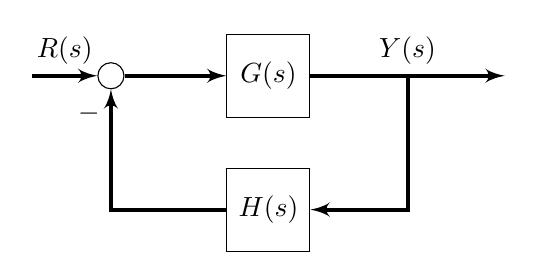
\begin{tikzpicture}[auto, node distance=2.5cm,>=latex']
					\node[input, name=rinput] (rinput) {};
					\node[sum, right of=rinput] (sum1) {};
					\node[block, right of=sum1,node distance=2cm] (Gs) {$G(s)$};
					\node[block, below of=Gs,node distance=1.7cm] (Hs) {$H(s)$};
					\node[output, right of=Gs,node distance=3cm] (output) {};
					\draw[->,line width = 0.5mm] (rinput) -- node[anchor=south]{$R(s)$} (sum1);
					\draw[->,line width = 0.5mm] (sum1) -- node[name=v1] {} (Gs);
					\draw[->,line width = 0.5mm] (Gs) -- node[name=y] {$Y(s)$} (output);
					\draw[->,line width = 0.5mm] (y) |- (Hs);	
					\draw[->,line width = 0.5mm] (Hs) -| node[pos=0.9] {$-$} (sum1);	
				\end{tikzpicture}
				\caption{Equivalencia de diagramas de bloques.}
				\label{fig:blockDiagram}
			\end{figure}

			\begin{figure}
				\centering
				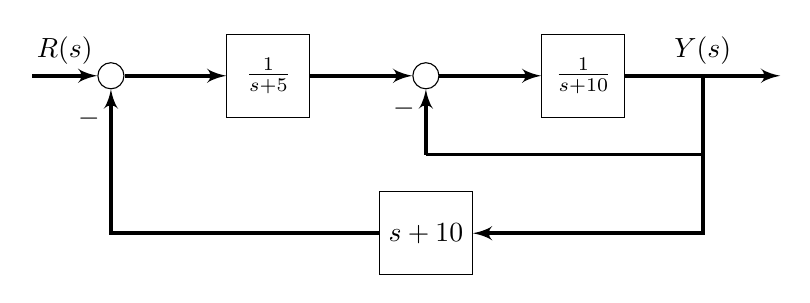
\begin{tikzpicture}[auto, node distance=2.5cm,>=latex']
					\node[input, name=rinput] (rinput) {};
					\node[sum, right of=rinput] (sum1) {};
					\node[block, right of=sum1,node distance=2cm] (sys1) {$\frac{1}{s+5}$};
					\node[sum, right of=sys1,node distance=2cm] (sum2) {};
					\node[block, right of=sum2,node distance=2cm] (sys2) {$\frac{1}{s+10}$};
					\node[block, below of=sum2, node distance=2cm] (sys3) {$s+10$};
					\node[output, right of=sys2] (output) {};
					\node[tmp, below of=sum2, node distance=1cm] (tmp2) {};
					\draw[->,line width=0.5mm] (rinput) -- node[anchor=south]{$R(s)$} (sum1);
					\draw[->,line width=0.5mm] (sum1) -- node[name=v1] {} (sys1);
					\draw[->,line width=0.5mm] (sys1) -- node[name=v2] {} (sum2);
					\draw[->,line width=0.5mm] (sum2) -- node[name=v3,anchor=north] {} (sys2);
					\draw[->,line width=0.5mm] (sys2) -- node[name=y] {$Y(s)$} (output);
					\draw[->,line width=0.5mm] (y) |- (sys3);	
					\draw[->,line width=0.5mm] (sys3) -| node[pos=0.9]{$-$} (sum1);	
					\draw[line width=0.5mm] (y) |- (tmp2);	
					\draw[->,line width=0.5mm] (tmp2) --  node[pos=0.7] {$-$}(sum2);	
				\end{tikzpicture}\\
				(a)\\
				\begin{tikzpicture}[auto, node distance=2.5cm,>=latex']
					\node[input, name=rinput] (rinput) {};
					\node[sum, right of=rinput] (sum1) {};
					\node[block, right of=sum1,node distance=2cm] (sys1) {$\frac{1}{s+5}$};
					\node[block, right of=sys1,node distance=2.5cm] (sys2) {$\frac{1}{s+11}$};
					\node[block, below of=v2, node distance=2cm] (sys3) {$s+10$};
					\node[output, right of=sys2] (output) {};
					\draw[->,line width=0.5mm] (rinput) -- node[anchor=south]{$R(s)$} (sum1);
					\draw[->,line width=0.5mm] (sum1) -- node[name=v1] {} (sys1);
					\draw[->,line width=0.5mm] (sys1) -- node[name=v2] {} (sys2);
					\draw[->,line width=0.5mm] (sys2) -- node[name=y] {$Y(s)$} (output);
					\draw[->,line width=0.5mm] (y) |- (sys3);	
					\draw[->,line width=0.5mm] (sys3) -| node[pos=0.9]{$-$} (sum1);	
				\end{tikzpicture}\\
				(b)\\
				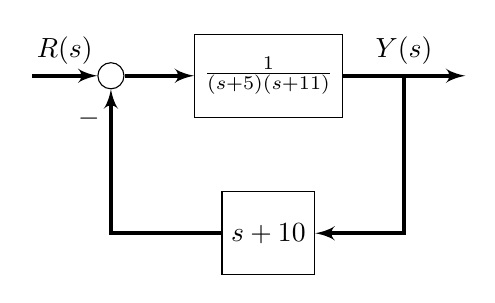
\begin{tikzpicture}[auto, node distance=2.5cm,>=latex']
					\node[input, name=rinput] (rinput) {};
					\node[sum, right of=rinput] (sum1) {};
					\node[block, right of=sum1,node distance=2cm] (sys1) {$\frac{1}{(s+5)(s+11)}$};
					\node[block, below of=sys1, node distance=2cm] (sys3) {$s+10$};
					\node[output, right of=sys1] (output) {};
					\draw[->,line width=0.5mm] (rinput) -- node[anchor=south]{$R(s)$} (sum1);
					\draw[->,line width=0.5mm] (sum1) -- node[name=v1] {} (sys1);
					\draw[->,line width=0.5mm] (sys1) -- node[name=y] {$Y(s)$} (output);
					\draw[->,line width=0.5mm] (y) |- (sys3);	
					\draw[->,line width=0.5mm] (sys3) -| node[pos=0.9]{$-$} (sum1);	
				\end{tikzpicture}\\
				(c)
				\caption{Simplificación del diagrama de bloque del problema 3.}
				\label{fig:blockDiagramSimplification}
			\end{figure}

			\item 4. Considere el sistema de control con retroalimentación negativa unitaria que posee la siguiente función de transferencia de lazo abierto:
			\begin{equation*}
				G_c(s)G(s) = \frac{K(s+1)(s+3)}{s(s-1)(s+2)}
			\end{equation*}
			Encuentre condiciones sobre el valor de la ganancia $K$ para que el sistema en lazo cerrado sea estable.\\
			Simplificando la función de transferencia se obtiene:
			\begin{equation*}
				G_c(s)G(s) = \frac{K(s^2+4Ks+3K)}{s^3+s^2-2s}
			\end{equation*}
			La función de transferencia de lazo cerrado es:
			\begin{align*}
				G_{cl}(s) = \frac{\frac{K(s^2+4Ks+3K)}{s^3+s^2-2s}}{1+\frac{K(s^2+4Ks+3K)}{s^3+s^2-2s}} = \frac{Ks^2+4Ks+3K}{s^3+(K+1)s^2+(4K-2)s+3K}
			\end{align*}
			Usando el criterio de Routh-Hurwitz se pueden hallar las condiciones sobre K para la estabilidad del sistema. El arreglo de Routh queda:
			\begin{table}[h]
				\centering
				\begin{tabular}{c|cc}
					$s^3$ & $1$ & $4K-2$\\
					$s^2$ & $K+1$ & $3K$\\
					$s^1$	& $a_1$\\
					$s^0$ & $a_0$
				\end{tabular}
			\end{table}
			\begin{align*}
				a_1 &= -\frac{1}{K+1}
				\begin{vmatrix}
					1 & 4K-2\\
					K+1 & 3K
				\end{vmatrix} = \frac{4K^2-K-2}{K+1}\\
				a_0 &= -\frac{1}{a_1}
				\begin{vmatrix}
					K+1 & 3K\\
					a_1 & 0
				\end{vmatrix} = -\frac{1}{a_1}(-3K a_1) = 3K
			\end{align*}
			La condición para que un sistema sea estable es que no existan cambios de signo en la primera columna del arreglo de Routh. Dicha columna corresponde a:
			\begin{equation*}
					\left\{1,\hspace*{2mm} K+1,\hspace*{2mm} \frac{4K^2-K-2}{K+1},\hspace*{2mm} 3K\right\}
			\end{equation*}
			Note que el primer valor es positivo, por lo que debemos buscar condiciones para que también lo sean. Del segundo valor se tiene la condición $K+1 > 0 \Rightarrow K>-1$. Para analizar el tercer valor se busca encontrar los valores críticos de $K$ tal que
			\begin{equation*}
				\frac{4K^2-K-2}{K+1} = 0\hspace*{3mm} \Rightarrow\hspace*{3mm} 4K^2-K-2=0\hspace*{3mm} \Rightarrow\hspace*{3mm} K = {0.8431, -0.5931}
			\end{equation*}
			Evaluando los dos valores posibles de $K$ en la primera columna del arreglo se tiene:
			\begin{align*}
				K &= 0.8431: \{1,\hspace*{2mm} 1.8431,\hspace*{2mm} 0,\hspace*{2mm} 2.5293\}\\
				K &= -0.5931: \{1,\hspace*{2mm} 0.4069,\hspace*{2mm} 0,\hspace*{2mm} -1.7793\}
			\end{align*}
			Nótese que en este caso para la primera solución se cumple que todos los valores son positivos, excepto el tercero. Para la segunda solución se obtiene que el último valor es negativo, por lo que no sería estable el sistema. Ahora, al modificar un poco la solución calculada se obtiene:
			\begin{align*}
				K &= 0.84: \{1,\hspace*{2mm} 1.84,\hspace*{2mm} -0.0096,\hspace*{2mm} 2.52\}\\
				K &= 0.85: \{1,\hspace*{2mm} 1.85,\hspace*{2mm} 0.0216,\hspace*{2mm} 2.55\}
			\end{align*}
			Note de nuevo que al disminuir un poco el valor de K, se obtienen un valor negativo, mientras que al aumentarlo se mantienen todos positivos. Por lo tanto, la condición para que el sistema sea estable es $K > 0.8431$.


			\item 5. Considere el sistema de lazo cerrado de la Fig. \ref{fig:steadyState}, donde
			\begin{equation*}
				G(s) = \frac{1}{s+10}, \hspace*{3mm} H(s) = \frac{14}{s^2+5s+6}
			\end{equation*}
			\begin{description}
				\item a. Calcule el valor del error en estado estacionario ante una referencia paso unitaria $R(s) = 1/s$.\\
				Para calcular el error de estado estacionario, primero se debe obtener la función de transferencia desde $R(s)$ hasta $E(s)$:
				\begin{align*}
					E(s) = R(s) - H(s)Y(s) = R(s) - G(s)H(s)E(s)\\
					E(s)\left( 1 + G(s)H(s) \right) = R(s)\\
					E(s) = \frac{1}{1+G(s)H(s)}R(s)
				\end{align*}
				Reemplazando las funciones de transferencia conocidas:
				\begin{equation*}
					E(s) = \frac{s^3+15s^2+56s+60}{s^3+15s^2+56s+74}R(s)
				\end{equation*}
				Usando el teorema del valor final:
				\begin{equation*}
					e_{ss} = \lim_{s \rightarrow 0}sE(s) = \lim_{s \rightarrow 0} s \frac{s^3+15s^2+56s+60}{s^3+15s^2+56s+74}\frac{1}{s} = \frac{60}{74} = 0.81081
				\end{equation*}

				\item b. Calcule el valor de la salida en estado estacionario ante un disturbio paso unitario $T_d(s) = 1/s$.\\
				Ahora, para calcular la función de transferencia desde el disturbio hasta la salida:
				\begin{align*}
					Y(s) = T_d(s) + G(s)H(s)Y(s)a\\
					Y(s) \left( 1 - G(s)H(s) \right) = T_d(s)\\
					Y(s) = \frac{1}{1-G(s)H(s)}T_d(s)
				\end{align*}
				Reemplazando las funciones de transferencia conocidas:
				\begin{equation*}
					Y(s) = \frac{s^3+15s^2+56s+60}{s^3+15s^2+56s+46} T_d(s)
				\end{equation*}
				Usando el teorema del valor final:
				\begin{equation*}
					y_{ss} = \lim_{s \rightarrow 0} sY(s) =  \lim_{s \rightarrow 0} s\frac{s^3+15s^2+56s+60}{s^3+15s^2+56s+46}\frac{1}{s} = \frac{60}{46} = 1.3043
				\end{equation*}

			\end{description}
			\begin{figure}
				\centering
				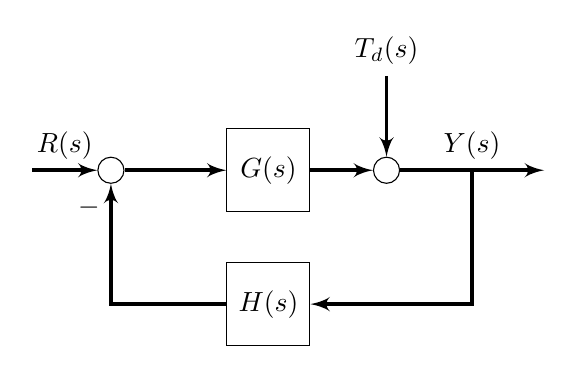
\begin{tikzpicture}[auto, node distance=2.5cm,>=latex']
					\node[input, name=rinput] (rinput) {};
					\node[sum, right of=rinput] (sum1) {};
					\node[block, right of=sum1,node distance=2cm] (Gs) {$G(s)$};
					\node[sum, right of=Gs,node distance=1.5cm] (sum2) {};
					\node[input, above of=sum2,name=tinput,node distance=1.2cm] (tinput) {};
					\node[block, below of=Gs,node distance=1.7cm] (Hs) {$H(s)$};
					\node[output, right of=sum2,node distance=2cm] (output) {};
					\draw[->,line width = 0.5mm] (rinput) -- node[anchor=south]{$R(s)$} (sum1);
					\draw[->,line width = 0.5mm] (sum1) -- node[name=v1] {} (Gs);
					\draw[->,line width = 0.5mm] (Gs) -- (sum2);
					\draw[->,line width = 0.5mm] (tinput) node[name=Td,anchor=south] {$T_d(s)$} -- (sum2);
					\draw[->,line width = 0.5mm] (sum2) -- node[name=y] {$Y(s)$} (output);
					\draw[->,line width = 0.5mm] (y) |- (Hs);	
					\draw[->,line width = 0.5mm] (Hs) -| node[pos=0.9] {$-$} (sum1);	
				\end{tikzpicture}
				\caption{Sistema de lazo cerrado sujeto a un disturbio.}
				\label{fig:steadyState}
			\end{figure}

			\item 6. Considere el sistema mostrado en la Fig. \ref{fig:itaeSystem}. Encuentre el valor de K tal que el sistema en lazo cerrado minimice el criterio de desempeño ITAE ante una entrada paso unitaria.\\

			Calculando la función de transferencia de lazo cerrado:
			\begin{equation*}
				\frac{Y(s)}{R(s)} = \frac{\frac{K}{s(s+5)}}{1+\frac{K}{s(s+5)}} = \frac{K}{s^2+5s+K}
			\end{equation*}
			La función obtenida de lazo cerrado se puede comparar directamente con la función de transferencia de un sistema óptimo ITAE de segundo orden:
			\begin{equation*}
				\frac{Y(s)}{R(s)} = \frac{\omega_n^2}{s^2 + 1.4 \omega_n s + \omega_n^2}
			\end{equation*}
			Comparando los coeficientes se tiene que:
			\begin{align*}
				1.4\omega_n = 5 \Rightarrow \omega_n = 3.5714\\
				K = \omega_n^2 = 12.7551
			\end{align*}

			\begin{figure}[h!]
				\centering
				% \includegraphics[width=7.5cm]{itaeSystem.eps}
				\begin{tikzpicture}[auto, node distance=2.5cm,>=latex']
					\node[input, name=rinput] (rinput) {};
					\node[sum, right of=rinput] (sum1) {};
					\node[block, right of=sum1,node distance=2cm] (sys1) {$K$};
					\node[block, right of=sys1,node distance=2.5cm] (sys2) {$\frac{1}{s(s+5)}$};
					\node[tmp, below of=v2, node distance=1.5cm] (tmp1) {};
					\node[output, right of=sys2] (output) {};
					\draw[->,line width=0.5mm] (rinput) -- node[anchor=south]{$R(s)$} (sum1);
					\draw[->,line width=0.5mm] (sum1) -- node[name=v1] {} (sys1);
					\draw[->,line width=0.5mm] (sys1) -- node[name=v2] {} (sys2);
					\draw[->,line width=0.5mm] (sys2) -- node[name=y] {$Y(s)$} (output);
					\draw[line width=0.5mm] (y) |- (tmp1);	
					\draw[->,line width=0.5mm] (tmp1) -| node[pos=0.9]{$-$} (sum1);	
				\end{tikzpicture}
				\caption{Sistema retroalimentado con controlador proporcional.}
				\label{fig:itaeSystem}
			\end{figure}

			\item 7. Considere el sistema mostrado en la Fig. \ref{fig:pidControl}. Se desea diseñar un control que disminuya el efecto de las perturbaciones $D(s)$. Diseñe un sistema de control tal que la respuesta a disturbio paso unitario desaparezca en menos de 3 s, con una oscilación cuya frecuencia natural sea $\omega_n = 4$ rad/s. Utilice una aproximación de polos dominantes.\\

			El controlador PID tiene la función de transferencia
			\begin{equation*}
				G_c(s) = \frac{K(as+1)(bs+1)}{s} = \frac{K(abs^2 + (a+b)s + 1)}{s}
			\end{equation*}
			La función de transferencia desde el disturbio hasta la salida es:
			\begin{align*}
				\frac{C(s)}{D(s)} &= \frac{G(s)}{1+G(s)G_c(s)} = \frac{s}{s(s^2+3.6s+9)+K(as+1)(bs+1)}\\
				&= \frac{s}{s^3 + (3.6+Kab)s^2 +(9+Ka+Kb)s + K}
			\end{align*}
			Se sabe que el disturbio debe desaparecer luego de 3s, por lo que $T_s = 3$. Entonces:
			\begin{equation*}
				T_s = \frac{4}{\zeta \omega_n},\hspace*{1mm} \omega_n = 4 \Rightarrow \zeta = \frac{1}{3}
			\end{equation*}
			Entonces el polinomio deseado que satisface éstos requerimientos es:
			\begin{equation*}
				s^2 + 2\zeta \omega_n s + \omega_n^2 = s^2 + \frac{8}{3}s + 16
			\end{equation*}
			Los polos se encuentran ubicados en $s = -1.333 \pm j3.7712$.
			Note que el polinomio obtenido para el sistema es de tercer orden. Por lo tanto agregamos un polo que se encuentre suficientemente alejado para no afectar de manera significativa la respuesta del sistema. En este caso se ubicará sobre el eje real a una distancia de 10 veces el valor de la parte real de los polos dominantes. Entonces el polinomio deseado incluyendo el tercer polo es:
			\begin{equation*}
				q(s) = (s^2 + \frac{8}{3}s + 16)(s+13) = s^3 + \frac{47}{3}s^2 + \frac{152}{3}s + 48
			\end{equation*}
			Igualando los coeficientes del polinomio deseado con el denominador de la función de transferencia $C(s)/D(s)$ se obtiene:
			\begin{align*}
				3.6 + Kab = \frac{47}{3} &\Rightarrow ab = 0.2514\\
				9 + K(a+b) = \frac{152}{3} &\Rightarrow a+b = 0.8681
			\end{align*}
			Entonces, el controlador PID diseñado queda:
			\begin{equation*}
				G_c(s) = \frac{48(0.2514s^2 + 0.8681s + 1)}{s}
			\end{equation*}
			La función de transferencia queda:
			\begin{equation*}
				\frac{C(s)}{D(s)} = \frac{s}{s^3+15.6672s^2+50.6688s+48}
			\end{equation*}
			Usando el teorema del valor final para encontrar el efecto de un disturbio paso unitario sobre la salida:
			\begin{equation*}
				c_{ss} = \lim_{s \rightarrow 0} sC(s) = \lim_{s \rightarrow 0} s \frac{s}{s^3+15.6672s^2+50.6688s+48} \frac{1}{s} = 0
			\end{equation*}
			Entonces, el control PID diseñado elimina totalmente el efecto del disturbio sobre la salida.
			\begin{figure}
				\centering
				% \includegraphics[width=13cm]{pidControl.eps}\\
				\begin{tikzpicture}[auto, node distance=2.5cm,>=latex']
					\node[input, name=rinput] (rinput) {};
					\node[sum, right of=rinput] (sum1) {};
					\node[block, right of=sum1,node distance=2cm] (sys1) {$\frac{K(as+1)(bs+1)}{s}$};
					\node[sum, right of=sys1,node distance=2.5cm] (sum2) {};
					\node[input, above of=sum2,name=dinput,node distance=1cm] (dinput) {};
					\node[block, right of=sum2,node distance=2cm] (sys2) {$\frac{1}{s^2+3.6s+9}$};
					\node[tmp, below of=v2, node distance=1.5cm] (tmp1) {};
					\node[output, right of=sys2] (output) {};
					\draw[->,line width=0.5mm] (rinput) -- node[anchor=south]{$R(s)$} (sum1);
					\draw[->,line width=0.5mm] (sum1) -- node[name=v1] {} (sys1);
					\draw[->,line width=0.5mm] (sys1) -- node[name=v2] {} (sum2);
					\draw[->,line width=0.5mm] (dinput)  node[anchor=south] {$D(s)$}--  (sum2);
					\draw[->,line width=0.5mm] (sum2) -- node[name=v3] {} (sys2);
					\draw[->,line width=0.5mm] (sys2) -- node[name=y] {$C(s)$} (output);
					\draw[line width=0.5mm] (y) |- (tmp1);	
					\draw[->,line width=0.5mm] (tmp1) -| node[pos=0.9]{$-$} (sum1);	
				\end{tikzpicture}
				\caption{Sistema de control PID}
				\label{fig:pidControl}
			\end{figure}
		\end{description}
\end{document}